\section{Motivation}

With upcoming high-luminosity running at CLAS12, the reduction of data can be beneficial for storage and online data transport.
In this work, we investigate Machine Learning (ML) approach to reduce the data footprint by compressing the pulse data using auto-encoder
type neural networks.

\subsection{Auto Encoders}

Autoencoders are a type of artificial neural network that is used to learn efficient codings of unlabeled data. They do this by learning two functions: an encoding function that transforms the input data, and a decoding function that recreates the input data from the encoded representation. The autoencoder learns an efficient representation (encoding) for a set of data, typically for dimensionality reduction. Variants exist, aiming to force the learned representations to assume useful properties.
Autoencoders are used for a variety of tasks, including:

\begin{figure}[h!]
\centering
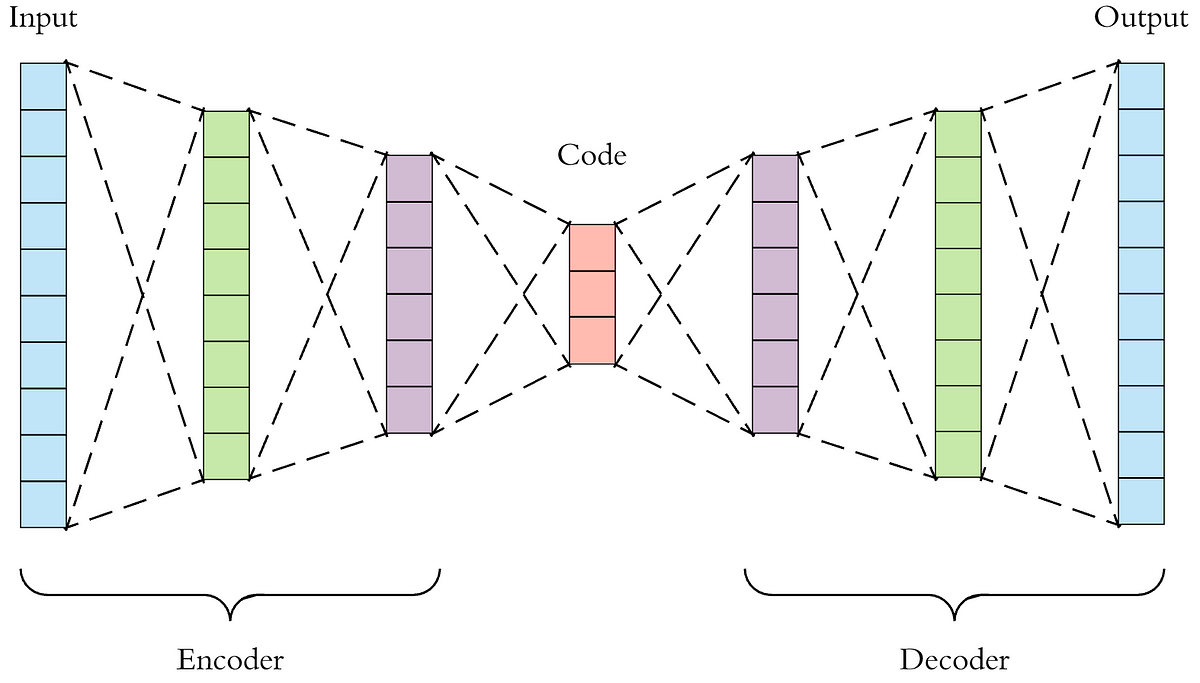
\includegraphics[width=0.6\columnwidth]{auto-encoders.png}
\caption{An autoencoder network architecture, consisting of encode part that is used to encode a more compact representation of the input into a latent space (Code) and
decoder part that reconstructs the latent space into a different representation of the input.} 
\label{fig:aeDiagram}
\end{figure}

\begin{itemize}
\item Image denoising: Autoencoders can be used to remove noise from images. This is done by first encoding the image into a lower-dimensional representation, and then decoding the representation back to an image. The noise is removed in the encoding process, so the decoded image is cleaner than the original image.
\item  Image compression: Autoencoders can be used to compress images. This is done by encoding the image into a lower-dimensional representation, which can then be stored more efficiently. When the encoded representation is decoded, the original image can be reconstructed.
\item Feature detection: Autoencoders can be used to detect features in data. This is done by learning an encoding representation that captures the most important features of the data. The encoded representation can then be used to identify similar data points.
\item Anomaly detection: Autoencoders can be used to detect anomalies in data. This is done by training the autoencoder on normal data. When new data is presented to the autoencoder, if the data is anomalous, the autoencoder will not be able to reconstruct the data as well as it can reconstruct normal data.
\end{itemize}
Autoencoders are a powerful tool for learning efficient representations of data. They are used for a variety of tasks, and their applications are still being explored. A typical architecture of an autoencoder is show in Figure~\ref{fig:aeDiagram}.


\subsection{Method}

In this paper, we use an autoencoder to compress the ADC pulse shape from the detectors. The input and output to the network are the pulse shape (represented by a vector of length 48), and the middle layer of the autoencoder will represent the compact representation of a pulse. The network is trained to reproduce the pulse in the output with good accuracy given the input pulse. In the compressions stage, this network will be used to run the network on raw data pulses and save the layer (called Code, see Figure~\ref{fig:aeDiagram}), which is smaller in size (in our studies factor of 4 smaller).
In the decompression stage, the saved vector will be read, and the second half of the network (called decoder, see Figure~\ref{fig:aeDiagram}) will run on the vector to reconstruct the full shape of the pulse. 



